\documentclass[a4paper]{article}

\usepackage{tecnico_relatorio}

\usepackage{textcomp}
\usepackage[hypcap]{caption} % makes \ref point to top of figures and tables
\usepackage{rotating}

\begin{document}
	\trSetImage{img/tecnico_logo}{6cm} % Logotipo do Técnico
	\trSetSubject{Co-Projecto HW/SW}
	\trSetType{Parte I}
	\trSetTitle{Compressão de Texto Usando Codificação de Huffman}
	
	\trSetBoxStyle{0.3}
	
	\trSetAuthorNr{2}
	
	\trSetAuthors
		{
		\begin{center}
		Gonçalo Ribeiro
		
		73294
		\end{center}
		}{
		\begin{center}
		Luís Fiolhais
		
		74171
		\end{center}
		}

	\trSetProfessor{Prof. Horácio Neto}
	
	\trMakeCover
	
	\tableofcontents
	\pagebreak
	
	\section{Introdução}
	
	Nesta parte do trabalho pretende-se criar um sistema constituído por um único processador MicroBlaze e um acelerador por hardware. O tema escolhido para o projecto é compressão de texto usando codificação de Huffman.
	
	Inicialmente começou-se por implementar o algoritmo de compressão em software. Depois de verificada a sua funcionalidade, o seu desempenho foi medido incluindo \textit{timers} no sistema e contabilizando o tempo despendido por cada parte do algoritmo para diversos ficheiros de exemplo. Com base nesta medição, escolheu-se uma parte do algoritmo para ser acelerada por hardware.
	
	O componente de hardware desenvolvido liga-se ao MicroBlaze através de uma interface FSL (\textit{Fast Simplex Link}). O acelerador foi desenhado e testado no Xilinx ISE (\textit{Integrated Synthesis Environment}) e subsequentemente integrado no sistema. O sistema foi testado e o desempenho foi novamente medido.
	
	\section{Codificação de Huffman}

	A codificação de Huffman é um método de compressão que consiste em encontrar uma representação alternativa---um \emph{código}---para cada \emph{símbolo} do alfabeto dos dados a comprimir. A compressão resulta do facto de o código escolhido para um dado símbolo ser tanto mais curto quanto maior for a frequência absoluta desse símbolo nos dados. A símbolos mais raros são atribuídos códigos mais longos. Os códigos encontrados têm uma propriedade importante: nenhum código é prefixo de outro código. Isto permite que durante processo de descompressão não haja qualquer ambiguidade.
	
	Os passos necessários ao algoritmo de compressão são os seguintes:
	
	\begin{enumerate}
	\item obter as frequências absolutas de cada símbolo
	\item construir uma árvore de Huffman
	\item codificar os dados
	\end{enumerate}
	
	O primeiro passo consiste em contar o número de ocorrências de cada símbolo até encontrar o fim do ficheiro. O segundo passo é criar uma \emph{trie} a partir das frequências obtidas no primeiro passo. Por último o ficheiro é comprimido fazendo uso da árvore criada.
	
	O processo de criação da árvore de Huffman é:
	
	\begin{enumerate}
	\item criar um nó para cada símbolo do alfabeto, em que se inclui a frequência desse símbolo
	\item enquanto existir mais que uma árvore
		\begin{enumerate}
		\item encontrar as duas árvores cuja raiz tem menor frequência
		\item tornar essas árvores descendentes de um novo nó, cuja frequência é a soma das frequências das raízes das duas árvores
		\end{enumerate}
	\end{enumerate}
	
	No final sobra apenas uma árvore que contém os nós correspondentes a cada símbolo. A localização desses nós na \textit{trie} dá-nos o código desse símbolo.
	
	\subsection*{Exemplo}
	
	Tome-se como exemplo o ficheiro \texttt{ABBCCCDDDD<EOF>}, em que \texttt{<EOF>} é o carácter terminador do ficheiro. Na \autoref{fig:huffman_tree_example} pode ver-se um exemplo de árvore de Huffman criada para este ficheiro.
	
	\begin{figure}[h]
		\centering
		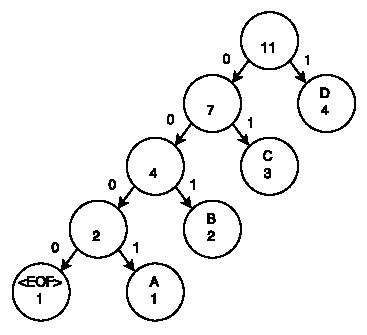
\includegraphics[width=.65\textwidth]{img/huffman_tree_example}
		\caption{Exemplo de uma árvore de Huffman}
		\label{fig:huffman_tree_example}
	\end{figure}
	
	Os códigos para cada carácter obtêm-se percorrendo a \textit{trie} da raiz até à folha que contem o respectivo carácter. Cada vez que se passa para um filho à esquerda adicionamos o bit 0 à codificação; cada vez que se segue para um filho à direita adiciona-se um bit com o valor 1. Assim por exemplo o código de \texttt{A} é \texttt{0001}, o de \texttt{C} é \texttt{01} e o de \texttt{D} é \texttt{1}. É de notar que, tal como previsto, os caracteres que ocorrem menos vezes têm códigos mais curtos.
	
	\section{Software}
	
	\section{Acelerador}
	
	\section{Resultados}
	
	\section{Testes e Simulações}
	
	\section{Dificuldades}	
	
	\section{Conclusão}


	% references

\end{document}








